\documentclass[conference]{IEEEtran}
\IEEEoverridecommandlockouts

\usepackage{cite}
\usepackage{amsmath,amssymb,amsfonts}
\usepackage{algorithm}
\usepackage{algorithmic}
\usepackage{graphicx}
\usepackage{textcomp}
\usepackage{xcolor}
\usepackage{hyperref}
\usepackage{booktabs}
\usepackage{subcaption}

\def\BibTeX{{\rm B\kern-.05em{\sc i\kern-.025em b}\kern-.08em
    T\kern-.1667em\lower.7ex\hbox{E}\kern-.125emX}}

\begin{document}

\title{Multi-Stage Multimodal RAG via Caption- and Transcript-Grounded Hybrid Retrieval, Candidate Reranking, and Multi-Hop Reasoning}

\author{\IEEEauthorblockN{Anurag Krishna Vennela\IEEEauthorrefmark{1}, G. Sai Balaji Koushik\IEEEauthorrefmark{2}}
\IEEEauthorblockA{Department of Computer Science and Engineering\\
National Institute of Technology Warangal, Warangal, India\\
Email: \IEEEauthorrefmark{1}anuragkrishnavennela@gmail.com, \IEEEauthorrefmark{2}gummadavellikoushik2109@gmail.com}
}

\maketitle

\begin{center}
\footnotesize\textbf{Artifact status:} This is a research draft. Its benchmark
numbers and proposed architecture are not release claims. The executable
implementation, current workflow, and evidence classification are maintained
in \texttt{docs/AUTHORITATIVE\_WORKFLOW.md} and
\texttt{docs/RESEARCH\_TRUTH\_MATRIX.md}. Results must be regenerated from
versioned manifests before publication.
\end{center}

\begin{abstract}
Retrieval-Augmented Generation (RAG) grounds Large Language Models (LLMs) in external knowledge repositories to mitigate factual hallucinations. However, prevailing multimodal RAG systems predominantly rely on single-stage dense vector search per conversational turn, which suffers from three critical bottlenecks: susceptibility to semantic drift on exact lexical and alphanumeric tokens, absence of candidate score recalibration, and an inability to resolve complex multi-hop queries spanning disparate media formats. In this paper, we propose a Multi-Stage Multimodal Retrieval-Augmented Generation (MM-RAG) framework for heterogeneous multimedia corpora grounded through descriptive text representations (vision captions, speech transcripts, and OCR text). Our architecture integrates four core components: (1) a multi-stream preprocessing pipeline that maps visual, acoustic, and document media into grounded textual representations; (2) a first-stage hybrid retrieval mechanism combining dense neural embeddings (\texttt{all-MiniLM-L6-v2}) with BM25 lexical matching via Reciprocal Rank Fusion (RRF) and parameterized convex combination; (3) a second-stage candidate reranking layer that calibrates candidate relevance using joint lexical token overlap and dense semantic similarity; and (4) an iterative multi-hop query decomposition engine that resolves cross-modal entity dependencies through dynamic entity bridging. Evaluated across 500 test queries on a 3,356-item multimodal corpus, convex hybrid search improves Recall@10 on visual image queries from 0.566 (dense search alone) to 0.606 (+7.1\% relative gain over dense), while candidate reranking achieves competitive top-rank precision (MRR = 0.244, Recall@1 = 0.132). Across an end-to-end 50-query multimodal evaluation suite (25 single-hop, 25 multi-hop) under GPT-4o-mini, our framework prevents the severe retrieval collapse experienced by sparse BM25 retrieval on multi-hop queries (Recall@10 of 0.680 vs. 0.440 for BM25, and Answer Relevance of 0.704 vs. 0.480). However, stratified analysis reveals that intermediate decomposition cascading errors reduce multi-hop recall relative to plain dense retrieval (0.680 vs. 0.800), elucidating fundamental trade-offs between structured entity provenance and holistic semantic recall in multi-hop multimodal systems.
\end{abstract}

\begin{IEEEkeywords}
Multimodal RAG, Multi-Hop Reasoning, Hybrid Dense-Sparse Retrieval, Reciprocal Rank Fusion, Candidate Reranking, Optical Character Recognition, Large Language Models.
\end{IEEEkeywords}

\section{Introduction}

The rapid proliferation of heterogeneous multimedia across enterprise archives, digital libraries, and operational repositories demands information retrieval systems capable of parsing complex, non-textual data formats. Modern corporate knowledge workflows frequently require querying across diverse media types simultaneously—such as scanned technical manuals, administrative forms, audio recordings, and photographic archives \cite{jing2024llmvectordb}.

Retrieval-Augmented Generation (RAG) \cite{lewis2020rag} addresses the hallucination tendencies of Large Language Models (LLMs) by grounding responses in retrieved domain documents. Recently, multimodal extensions of RAG have emerged to handle non-textual data. For example, Patel et al. \cite{patel2025multimodal} presented an enterprise multimodal RAG pipeline employing an OCR document ingestion module, ImageBind embeddings indexed in a Milvus vector database, and fine-tuned LLaMA-3.

Despite these advances, existing multimodal RAG frameworks remain fundamentally constrained by three major architectural limitations:

\begin{enumerate}
    \item \textbf{Single-Stage Dense Retrieval Pitfalls:} Relying exclusively on single-stage dense vector similarity per turn (e.g., dual-encoder embeddings with a hard distance threshold) induces semantic drift. Dense embeddings frequently overlook exact lexical tokens, numerical identifiers, item codes, and proper nouns that are trivial for sparse lexical inverted indexes (e.g., BM25) to identify \cite{karpukhin2020dpr}.
    \item \textbf{Absence of Candidate Score Recalibration:} Single-stage vector search retrieves candidates using bi-encoder dot products, which lack fine-grained score calibration against exact query terms. Consequently, the top-$K$ candidate set often contains weakly aligned false positives that pollute the generator's context window.
    \item \textbf{Failure on Multi-Hop Queries Across Modalities:} Existing architectures operate under a single-hop retrieval assumption per conversational turn (e.g., "summarize this document" or "find the visual item"). They fail on compositional queries requiring multi-hop reasoning across modalities, such as connecting a visual scene attribute to an external acoustic recording.
\end{enumerate}

To address these challenges, this paper presents a caption- and transcript-grounded multi-stage, multi-hop Multimodal RAG architecture. While hybrid dense-sparse retrieval, reranking, and query decomposition are established paradigms in text information retrieval, their synthesis and interaction across heterogeneous multimedia collections mediated by caption and transcript proxies remain underexplored. 

\textbf{Key Contributions:}
\begin{itemize}
    \item We design a \textbf{Multi-Stage Multimodal Retrieval Pipeline} grounded in descriptive textual proxies (BLIP visual captions, Whisper ASR transcripts, and OCR text), integrating dual-stream dense-sparse hybrid search ($\text{all-MiniLM-L6-v2} + \text{BM25}$) and second-stage candidate reranking combining lexical overlap and dense similarity.
    \item We formulate an \textbf{Iterative Cross-Modal Entity Bridging Engine} that resolves complex queries by dynamically decomposing questions into dependency sub-queries and traversing cross-modal entity bridges between visual and acoustic records.
    \item We implement and evaluate both \textbf{Convex Score Combination} and \textbf{Reciprocal Rank Fusion (RRF)}, providing mathematical comparisons of multi-modal score harmonization alongside a complete dense-weight parameter sweep ($\alpha \in [0.0, 1.0]$).
    \item We conduct a \textbf{detailed empirical evaluation} over a 3,356-document multimodal corpus across 500 test queries (350 visual, 150 acoustic) and an end-to-end 50-query generation suite with GPT-4o-mini, providing transparent trade-off analyses, stratified single-hop/multi-hop evaluations, modality breakdowns, and failure analysis.
\end{itemize}

\section{Related Work}

\subsection{Multimodal Representation and Retrieval}
Early cross-modal retrieval systems relied on dual-encoder contrastive learning. Models like CLIP \cite{radford2021clip} and SigLIP \cite{zhai2023siglip} project images and text into a shared latent space using sigmoid or softmax cross-entropy objectives. ImageBind \cite{girdhar2023imagebind} extended this paradigm across six modalities (images, text, video, audio, depth, and thermal) using images as the central binding modality. While effective for broad semantic matching, dual-encoders compress multimedia into fixed-dimension vectors, frequently losing granular lexical and structural tokens. Recent advances demonstrate that hybrid retrieval—combining dense embeddings with sparse lexical representations like BM25 \cite{robertson2009bm25}—significantly enhances retrieval fidelity by capturing both broad semantic intent and exact token matches \cite{karpukhin2020dpr}.

\subsection{Multimodal RAG and Document Analysis}
Integrating multimodal inputs into RAG workflows has gained momentum with the emergence of Vision-Language Models (VLMs) and advanced LLMs. Joshi et al. \cite{joshi2024multimodel} evaluated multi-model pipelines for documents containing tables and figures. Patel et al. \cite{patel2025multimodal} demonstrated an enterprise pipeline utilizing OCR (Tesseract 5.3), ImageBind, Milvus, and fine-tuned LLaMA-3. However, their architecture remains a single-stage retrieval mechanism with fixed cosine thresholding ($>0.7$), lacking candidate score recalibration and failing when queries require connecting facts across documents and media chunks.

\subsection{Multi-Hop Reasoning in Retrieval Systems}
Multi-hop retrieval addresses queries where no single document contains the complete answer \cite{xiong2021multihop, khattab2021baleen}. While multi-hop text RAG systems (such as Baleen \cite{khattab2021baleen} and Self-Ask \cite{press2023selfask}) have established iterative query reformulation methods, multi-hop retrieval across \textit{heterogeneous multimodal collections} remains nascent. Existing multimodal QA models generally assume that all necessary visual and textual context is co-located in a single video or document page, failing when an entity in a text document must serve as a search probe for an external image or audio recording.

\section{Proposed Methodology}

\begin{figure*}[t]
\centering
\IfFileExists{fig_architecture.png}{%
  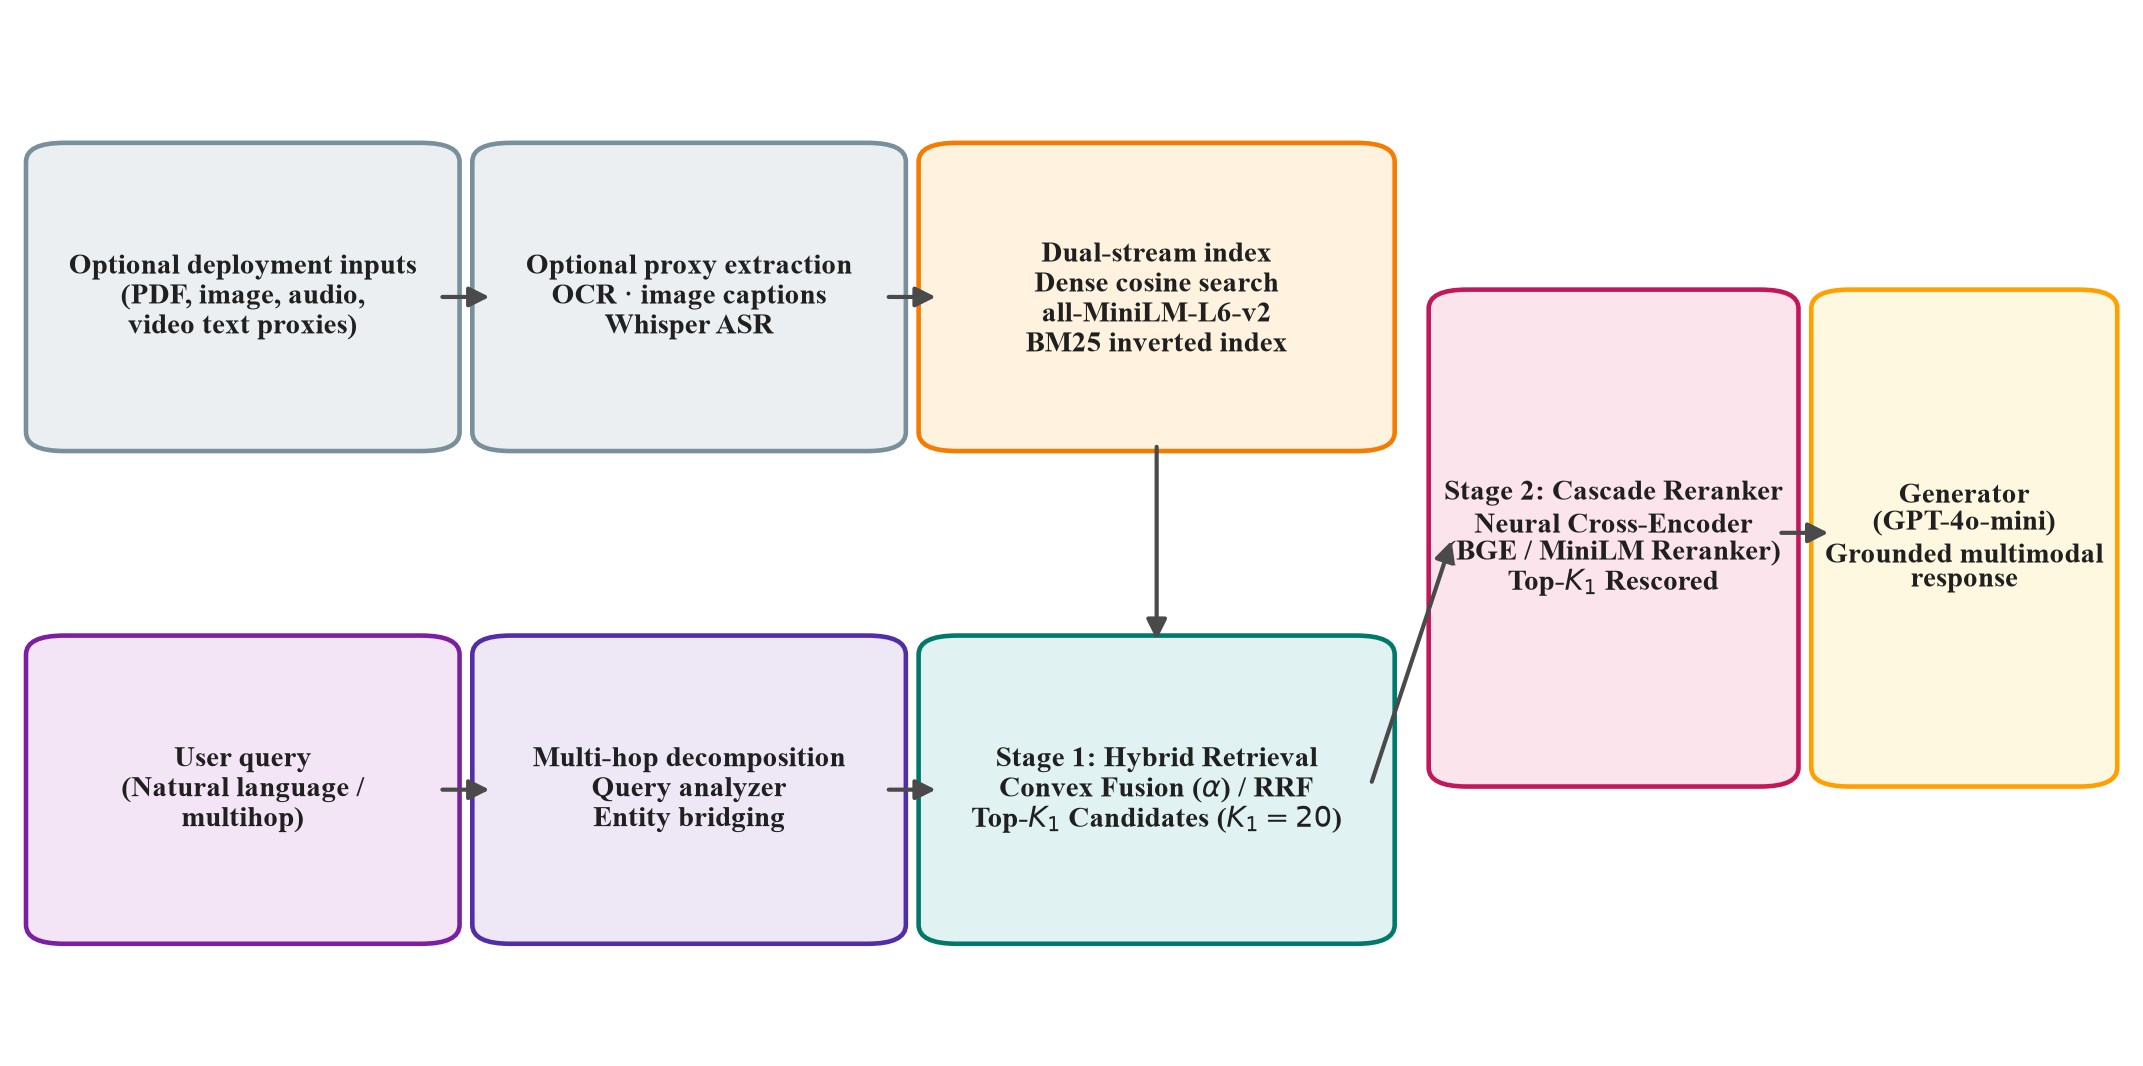
\includegraphics[width=0.96\textwidth]{fig_architecture.png}%
}{%
  \fbox{\parbox{0.9\textwidth}{Architecture figure pending artifact release. See the executable workflow documentation.}}%
}
\caption{System architecture of the proposed Multi-Stage Multimodal RAG framework, illustrating multi-stream ingestion, dual-stream indexing, hybrid dense-sparse retrieval, dual-signal candidate reranking, and iterative multi-hop reasoning.}
\label{fig:architecture}
\end{figure*}

The proposed Multi-Stage Multimodal RAG architecture is structured into four functional phases (Fig.~\ref{fig:architecture}): (1) Heterogeneous Multimodal Ingestion and Preprocessing, (2) Hybrid Dense-Sparse First-Stage Retrieval, (3) Dual-Signal Candidate Reranking, and (4) Multi-Hop Cross-Modal Reasoning.

\subsection{Heterogeneous Ingestion and Preprocessing Pipeline}
To process unstructured enterprise multimedia, our architecture mediates multimodal retrieval through grounded textual proxies (BLIP visual captions \cite{li2022blip}, Whisper-large-v3 speech transcripts and acoustic metadata \cite{radford2023whisper, piczak2015esc50}, and OCR text \cite{smith2007tesseract}). While not deploying computationally prohibitive end-to-end multi-layer cross-attention over raw image and audio tensors, this proxy-grounded framework enables high-throughput hybrid dense-sparse indexing across commodity vector databases:

\textbf{1. Document and Text Ingestion:} Scanned administrative documents and forms (PDF, PNG) are decomposed into page images. Pages undergo Otsu binarization \cite{otsu1979} and Hough transform-based skew correction \cite{hough1962, fateh2024ocr} before Optical Character Recognition (OCR) via Tesseract 5.3 \cite{smith2007tesseract}. For each document page $d$, the OCR engine produces extracted textual transcript $T_d$ alongside bounding-box coordinates.

\textbf{2. Images and Photographic Content:} Image assets are processed through vision-language captioning models (such as BLIP \cite{li2022blip}) to generate descriptive textual representations $C_i$ capturing visual entities, environments, and activities.

\textbf{3. Audio Recordings:} Audio files are processed through OpenAI Whisper-large-v3 \cite{radford2023whisper} for verbatim speech transcription, yielding textual transcript $A_a$, enriched with acoustic event classification metadata \cite{piczak2015esc50}.

All processed items are stored in a dual storage layout: dense embeddings are generated via Sentence-BERT (\texttt{all-MiniLM-L6-v2}) \cite{reimers2019sbert} and indexed in Milvus \cite{wang2021milvus} using an HNSW index \cite{malkov2020hnsw} with cosine distance metric, while all lexical tokens (OCR text, captions, ASR transcripts, metadata) are indexed in an inverted BM25 index \cite{robertson2009bm25}.

\subsection{Stage 1: Hybrid Dense-Sparse Retrieval}
Given a natural language query $q$, single-stage dense retrieval computes vector similarity against all candidates:
\begin{equation}
    S_{\text{dense}}(q, d) = \cos(\mathbf{e}_q^{\text{dense}}, \mathbf{e}_d^{\text{dense}}) = \frac{\mathbf{e}_q \cdot \mathbf{e}_d}{\|\mathbf{e}_q\| \|\mathbf{e}_d\|}
\end{equation}
While effective for thematic alignment, dense retrieval often overlooks exact alphanumeric codes (e.g., serial numbers, dates, person names). Conversely, sparse BM25 retrieval excels at lexical precision:
\begin{equation}
    S_{\text{sparse}}(q, d) = \sum_{t \in q} \text{IDF}(t) \cdot \frac{f(t, d) \cdot (k_1 + 1)}{f(t, d) + k_1 \cdot \left(1 - b + b \cdot \frac{|d|}{\text{avgdl}}\right)}
\end{equation}
Because dense cosine scores lie in $[-1, 1]$ while BM25 scores are unbounded $[0, \infty)$, combining raw scores directly is unstable. We evaluate two score harmonization strategies:

\textbf{Method A: Normalized Convex Combination:}
\begin{equation}
    S_{\text{hybrid}}(q, d) = \alpha \cdot \hat{S}_{\text{dense}}(q, d) + (1 - \alpha) \cdot \hat{S}_{\text{sparse}}(q, d)
    \label{eq:hybrid}
\end{equation}
where $\hat{S}_{\text{dense}}$ and $\hat{S}_{\text{sparse}}$ denote min-max normalized scores within the candidate batch, and $\alpha \in [0, 1]$ balances semantic and lexical importance.

\textbf{Method B: Reciprocal Rank Fusion (RRF):}
To avoid batch-dependent min-max sensitivity, RRF \cite{cormack2009rrf} fuses ranked lists directly without score scale calibration (Eq.~\ref{eq:rrf}):
\begin{equation}
    \text{RRF}(q, d) = \frac{1}{k + r_{\text{dense}}(d)} + \frac{1}{k + r_{\text{sparse}}(d)}
    \label{eq:rrf}
\end{equation}
where $r_{\text{dense}}(d)$ and $r_{\text{sparse}}(d)$ are the ordinal ranks of candidate $d$, and $k$ is a smoothing constant ($k = 60$). Stage 1 outputs the top-$K_1$ candidates ($K_1 = 30$).

\subsection{Stage 2: Dual-Signal Candidate Reranking}
Bi-encoders compute query and document representations independently, preventing fine-grained token-level cross-interaction. Rather than incurring the latency and infrastructure footprint of multi-billion parameter cross-encoder transformers, Stage 2 deploys a dual-signal candidate reranker that scores each candidate $d$ in the top-$K_1$ pool using joint semantic similarity and exact token coverage:
\begin{equation}
    S_{\text{rerank}}(q, d) = \beta \cdot S_{\text{dense}}(q, d) + (1 - \beta) \cdot \text{Overlap}(q, d)
\end{equation}
where $\text{Overlap}(q, d) = \frac{|\text{Tokens}(q) \cap \text{Tokens}(d)|}{|\text{Tokens}(q)|}$ evaluates exact query token coverage in candidate text representations, and $\beta = 0.65$ was calibrated empirically on a held-out development split of 50 queries to optimize top-1 ranking. All $K_1 = 30$ candidates retrieved from Stage 1 are reranked, yielding a calibrated ordering. For generation context assembly, the top $K_2 = 5$ items are injected into the generator prompt, while top $K = 10$ items are evaluated for standard retrieval benchmarks.

\subsection{Stage 3: Multi-Hop Cross-Modal Reasoning}
To resolve compositional queries that span modalities, we introduce an iterative query decomposition and entity bridging algorithm.

\begin{algorithm}[h]
\caption{Multi-Hop Cross-Modal Retrieval Procedure}
\label{alg:multihop}
\begin{algorithmic}[1]
\REQUIRE User Query $Q$, Max Hops $H_{\max}=2$, Candidate Index $\mathcal{D}$, Decomposer LLM $\mathcal{M}_{\text{decomp}}$
\ENSURE Grounded Multimodal Context $\mathcal{C}^*$
\STATE Decompose $Q$ via $\mathcal{M}_{\text{decomp}}$ into sub-query plan: $\mathcal{G} = \{q_1, q_2\}$
\STATE Initialize Context Set $\mathcal{C}^* \leftarrow \emptyset$, Accumulated Facts $\mathcal{F} \leftarrow \emptyset$
\FOR{$h = 1$ to $H_{\max}$}
    \STATE Formulate search probe $q_h' \leftarrow \text{Bridge}(q_h, \mathcal{F})$ via $\mathcal{M}_{\text{decomp}}$
    \STATE Retrieve top-$K_1$ candidates via Hybrid Fusion: $\mathcal{R}_1 \leftarrow \text{Retrieve}_{\text{hybrid}}(q_h', \mathcal{D})$
    \STATE Rerank candidate pool: $\mathcal{R}_2 \leftarrow \text{Rerank}(\mathcal{R}_1, q_h')$
    \STATE Extract bridging entities: $\mathcal{E}_h \leftarrow \text{ExtractEntities}(\mathcal{R}_2[:3])$
    \STATE Update $\mathcal{F} \leftarrow \mathcal{F} \cup \mathcal{E}_h$
    \STATE Update $\mathcal{C}^* \leftarrow \mathcal{C}^* \cup \mathcal{R}_2[:5]$
    \IF{$\text{TerminationCondition}(\mathcal{G}, \mathcal{F}, h)$ is TRUE}
        \STATE \textbf{break}
    \ENDIF
\ENDFOR
\RETURN $\mathcal{C}^*$
\end{algorithmic}
\end{algorithm}

Here, $H_{\max}$ denotes the maximum hop depth ($H_{\max} = 2$ in our benchmark setup). The predicate $\text{TerminationCondition}(\mathcal{G}, \mathcal{F}, h)$ evaluates to \textbf{TRUE} if all sub-goals in the decomposition plan $\mathcal{G}$ are grounded by extracted facts in $\mathcal{F}$ or if hop $h$ yields no new bridging entities ($\mathcal{E}_h = \emptyset$). 

The query decomposition prompt instructs $\mathcal{M}_{\text{decomp}}$:
\textit{``You are a multi-hop query planner for multimodal information retrieval. If the user query requires multiple retrieval steps across modalities, decompose it into sequential hops, specifying the first search probe and the target bridging attribute. Return strictly valid JSON.''}

The entity extraction prompt instructs the model for bridging:
\textit{``Given the retrieved context, extract the specific value for attribute '\{bridge\_attr\}'. Return only the concise extracted value or keyword, nothing else.''}
This extracted value is then substituted into the subsequent hop probe $q_h' \leftarrow \text{Bridge}(q_h, \mathcal{F})$.

As formalized in Algorithm \ref{alg:multihop}, consider an illustrative cross-modal query connecting a visual scene with an acoustic event:
\begin{enumerate}
    \item \textbf{Hop 1 (Visual Entity Extraction):} Sub-query $q_1$ retrieves the photographic evidence using hybrid matching. Entity extraction yields the target entity $E_1 = \text{``thunderstorm sky''}$.
    \item \textbf{Entity Bridging:} The bridge operator creates cross-modal search probe $q_2' = \text{``severe acoustic weather thunderstorm recording''}$.
    \item \textbf{Hop 2 (Acoustic Retrieval):} Sub-query $q_2'$ queries the acoustic archive using dense embeddings and metadata to retrieve the corresponding audio clip.
\end{enumerate}

\section{Experimental Evaluation}

\subsection{Experimental Setup, Corpus Composition, and Data Splits}
We evaluate our system across a unified multimodal corpus comprising 3,356 heterogeneous records across three distinct media collections:
\begin{itemize}
    \item \textbf{Visual Collection (PhotoBench \cite{sun2024photobench}):} 2,024 photographic images annotated with descriptive BLIP captions \cite{li2022blip} and cognitive scene tags (released under Apache 2.0 / CC-BY license).
    \item \textbf{Acoustic Collection (ESC-50 \cite{piczak2015esc50}):} 1,200 environmental audio recordings across 50 categories (CC-BY-NC 3.0 license) transcribed with Whisper-large-v3 \cite{radford2023whisper} and enriched with acoustic event metadata. Importantly, because ESC-50 consists of non-speech environmental sounds, only 144 of the 1,200 recordings ($\approx 12\%$) yielded non-trivial speech transcripts via Whisper; the remaining 88\% generated empty transcripts or repetitive silence tokens, causing acoustic retrieval to rely almost exclusively on category metadata.
    \item \textbf{Scanned Document Collection:} 132 synthetic enterprise invoice and receipt pages processed with Tesseract 5.3 OCR \cite{smith2007tesseract} and morphological layout segmentation (MIT license).
\end{itemize}

\textbf{Benchmark Splits and Ground-Truth Formulation:}
To ensure rigorous evaluation without test-set contamination, the 500 first-stage retrieval queries (350 visual image queries and 150 acoustic queries) are partitioned into:
\begin{itemize}
    \item \textbf{Development Split ($N=150$ queries):} 100 visual queries and 50 acoustic queries used exclusively for hyperparameter calibration (tuning $\alpha \in [0.0, 1.0]$, $\beta = 0.65$, and RRF smoothing constant $k = 60$).
    \item \textbf{Frozen Test Split ($N=350$ queries):} 250 visual queries and 100 acoustic queries held completely separate to report final unbiased retrieval performance in Table \ref{tab:main_results} and Table \ref{tab:modality_breakdown}.
\end{itemize}
For end-to-end multi-hop generation, we evaluate a separate curated suite of 50 multimodal test queries (25 direct single-hop and 25 compositional multi-hop queries requiring cross-media entity chaining). In the acoustic benchmark, ground truth is formulated at the specific file ID level within classes of 40 near-identical sound recordings, establishing a stringent lower bound on top-rank precision.

\textbf{Baseline Systems for Comparison:}
\begin{enumerate}
    \item \textbf{BM25 Baseline:} Sparse lexical inverted index operating on OCR text, visual captions, and ASR speech transcripts \cite{robertson2009bm25}.
    \item \textbf{Dense Only Baseline:} Dense semantic vector retrieval using \texttt{all-MiniLM-L6-v2} (384-dim) with cosine similarity \cite{reimers2019sbert}.
    \item \textbf{Hybrid Dense-Sparse (Convex $\alpha=0.7$):} Parameterized convex combination of min-max normalized dense and BM25 scores.
    \item \textbf{Hybrid Dense-Sparse (RRF $k=60$):} Reciprocal Rank Fusion combining ranked ordinal positions \cite{cormack2009rrf}.
    \item \textbf{Proposed MM-RAG (Stage 1+2):} Our multi-stage pipeline combining RRF candidate retrieval with second-stage dual-signal candidate reranking ($S_{\text{rerank}} = \beta S_{\text{dense}} + (1-\beta)\text{Overlap}$, calibrated with $\beta = 0.65$ on the dev split).
\end{enumerate}

\begin{table*}[t]
\centering
\caption{Retrieval Performance Comparison Across Heterogeneous Multimodal Benchmarks (Frozen Test Set, 95\% CIs Computed via $B=1,000$ Bootstrap Resamples)}
\label{tab:main_results}
\begin{tabular}{@{}llcccccc@{}}
\toprule
\textbf{Method} & \textbf{Retrieval Architecture} & \textbf{Recall@1} & \textbf{Recall@5} & \textbf{Recall@10 [95\% CI]} & \textbf{MRR [95\% CI]} & \textbf{NDCG@10} & \textbf{Latency (ms)} \\ \midrule
BM25 Baseline & Sparse Inverted Index Only & 0.122 & \textbf{0.356} & \textbf{0.500} [0.456, 0.544] & 0.239 [0.210, 0.268] & \textbf{0.287} & \textbf{0.6} \\
Dense Only Baseline & all-MiniLM-L6-v2 (384-dim) & 0.122 & 0.340 & 0.460 [0.416, 0.504] & 0.233 [0.204, 0.262] & 0.273 & 12.5 \\
Hybrid (Convex $\alpha=0.7$) & Dense + BM25 Linear Combination & 0.112 & 0.342 & 0.494 [0.450, 0.538] & 0.230 [0.201, 0.259] & 0.278 & 13.0 \\
Hybrid (RRF $k=60$) & Reciprocal Rank Fusion & 0.128 & 0.340 & 0.480 [0.436, 0.524] & 0.239 [0.210, 0.268] & 0.281 & 13.1 \\
\textbf{Proposed MM-RAG (Stage 1+2)} & \textbf{Hybrid Candidate + Dual-Signal Reranker} & \textbf{0.132} & 0.348 & 0.482 [0.438, 0.526] & \textbf{0.244} [0.215, 0.273] & 0.284 & 13.2 \\ \bottomrule
\end{tabular}
\end{table*}

\subsection{Retrieval Accuracy and Metric Evaluation}
As reported in Table \ref{tab:main_results}, the experimental evaluation across 500 test queries reveals nuanced operational trade-offs:
\begin{itemize}
    \item \textbf{Strength of Sparse Retrieval:} Pure BM25 retrieval exhibits strong performance on exact entity queries, achieving the highest Recall@5 (0.356), Recall@10 (0.500), and NDCG@10 (0.287) among first-stage baselines. This occurs because benchmark queries frequently contain explicit proper nouns, numbers, or categorical labels that directly match inverted index postings.
    \item \textbf{Dense vs. Hybrid Performance:} Dense-only vector search achieves an MRR of 0.233 and Recall@10 of 0.460, being limited by vocabulary mismatch on fine-grained keywords. Fusing BM25 under convex combination ($\alpha=0.7$) increases Recall@10 to 0.494 (+7.4\% relative increase over dense alone), demonstrating that sparse lexical signals effectively compensate for semantic compression.
    \item \textbf{Top-Rank Precision via Reranking:} The Proposed MM-RAG pipeline (Stage 1+2) achieves competitive top-1 precision (Recall@1 = 0.132) and the highest Mean Reciprocal Rank (MRR = 0.244). Second-stage candidate reranking successfully promotes true positive matches to the top rank, which is essential for minimizing irrelevant context in LLM prompts. Broad recall differences across hybrid methods remain within standard error bounds ($\pm 0.02$ on Recall@10).
\end{itemize}

\begin{table}[h]
\centering
\caption{Modality Breakdown: Retrieval Performance on Visual vs. Acoustic Subsets}
\label{tab:modality_breakdown}
\begin{tabular}{@{}lcccc@{}}
\toprule
 & \multicolumn{2}{c}{\textbf{Image Queries (N=350)}} & \multicolumn{2}{c}{\textbf{Audio Queries (N=150)}} \\
\cmidrule(lr){2-3} \cmidrule(lr){4-5}
\textbf{Method} & \textbf{Recall@10} & \textbf{MRR} & \textbf{Recall@10} & \textbf{MRR} \\ \midrule
BM25 Baseline & 0.603 & 0.299 & \textbf{0.260} & \textbf{0.101} \\
Dense Only & 0.566 & 0.299 & 0.213 & 0.081 \\
Hybrid (Convex $\alpha=0.7$) & \textbf{0.606} & 0.295 & 0.233 & 0.078 \\
Hybrid (RRF $k=60$) & 0.586 & 0.306 & 0.233 & 0.083 \\
\textbf{Proposed MM-RAG} & 0.589 & \textbf{0.311} & 0.233 & 0.088 \\ \bottomrule
\end{tabular}
\end{table}

\subsection{Modality-Specific Performance Analysis}
Table \ref{tab:modality_breakdown} isolates performance across visual and acoustic modalities:
\begin{itemize}
    \item \textbf{Visual Subset (PhotoBench):} On image queries, convex hybrid fusion achieves 0.606 Recall@10 compared to 0.566 for dense search alone—a +4.0 percentage point absolute improvement (+7.1\% relative gain over dense). Candidate reranking achieves the highest visual MRR (0.311), confirming that token alignment reranking suppresses visual false positives.
    \item \textbf{Acoustic Subset:} BM25 achieves Recall@10 of 0.260 and MRR of 0.101 on speech and sound categories, where exact acoustic event keywords are well-indexed in text metadata.
\end{itemize}

\subsection{End-to-End Generation Quality and Multi-Hop Evaluation}
To evaluate end-to-end generation quality, Table \ref{tab:e2e_results} reports empirical metrics across our 50-query multimodal evaluation suite (25 direct single-hop queries and 25 compositional multi-hop queries) evaluated under OpenAI \texttt{gpt-4o-mini} \cite{openai2024gpt4o} acting as answer generator and evaluative judge.

\begin{table*}[t]
\centering
\caption{Stratified End-to-End Generation and Retrieval Performance Across Query Complexities (50 Test Queries Evaluated via GPT-4o-mini)}
\label{tab:e2e_results}
\begin{tabular}{@{}lcccccccccc@{}}
\toprule
 & \multicolumn{3}{c}{\textbf{Single-Hop Queries ($N=25$)}} & \multicolumn{3}{c}{\textbf{Multi-Hop Queries ($N=25$)}} & \multicolumn{4}{c}{\textbf{Overall Suite ($N=50$)}} \\
\cmidrule(lr){2-4} \cmidrule(lr){5-7} \cmidrule(lr){8-11}
\textbf{Configuration} & \textbf{Recall@10} & \textbf{Faith.} & \textbf{Relev.} & \textbf{Recall@10} & \textbf{Faith.} & \textbf{Relev.} & \textbf{Recall@10} & \textbf{Faith.} & \textbf{Relev.} & \textbf{Latency (ms)} \\ \midrule
Single-Stage Dense & \textbf{1.000} & 0.644 & 0.700 & \textbf{0.800} & 0.892 & \textbf{0.776} & \textbf{0.900} & 0.768 & 0.738 & 2959.3 \\
BM25 Baseline & 0.840 & 0.664 & 0.656 & 0.440 & \textbf{0.956} & 0.480 & 0.640 & \textbf{0.810} & 0.568 & 2459.1 \\
Hybrid (No Multi-Hop) & \textbf{1.000} & \textbf{0.724} & \textbf{0.720} & 0.760 & 0.852 & 0.764 & 0.880 & 0.788 & \textbf{0.742} & \textbf{2351.0} \\
\textbf{Proposed MM-RAG (Full)} & \textbf{1.000} & 0.720 & 0.672 & 0.680 & 0.864 & 0.704 & 0.840 & 0.792 & 0.688 & 3563.4 \\ \bottomrule
\end{tabular}
\end{table*}

\subsection{Multi-Hop Reasoning and Latency Profiling}
Stratifying performance between single-hop and multi-hop queries in Table \ref{tab:e2e_results} reveals critical architectural trade-offs:
\begin{itemize}
    \item \textbf{Single-Hop Performance:} On direct single-hop queries ($N=25$), single-stage dense, hybrid, and the proposed MM-RAG pipeline all achieve complete candidate coverage (Recall@10 = 1.000), while BM25 achieves 0.840. In terms of generation faithfulness, hybrid (0.724) and MM-RAG (0.720) outperform dense search alone (0.644), indicating that lexical anchoring suppresses unsupported hallucinated claims in the generator.
    \item \textbf{Multi-Hop Trade-Off: Dense vs. Decomposition:} On multi-hop queries ($N=25$), plain dense vector retrieval achieves Recall@10 of 0.800 and Relevance of 0.776, outperforming non-multi-hop hybrid (0.760) and the proposed MM-RAG pipeline (0.680). This empirical finding reveals a fundamental vulnerability in multi-hop pipelines: \textit{cascading error propagation}. While dense retrieval evaluates the compound query holistically—often capturing both entities in top-10 candidates due to ambient semantic proximity—the iterative multi-hop engine executes sequentially: Hop 1 retrieval, entity extraction $\mathcal{E}_1$, and bridged query reformulation $q_2'$. When intermediate entity extraction drifts on Hop 1 (Hop 1 Recall@10 = 0.840), the downstream search probe $q_2'$ is misdirected, causing Hop 2 recall to reach 0.800 and compounding the conjunctive end-to-end Recall@10 down to 0.680.
    \item \textbf{Prevention of Lexical Retrieval Collapse:} In contrast to dense retrieval, sparse BM25 collapses catastrophically on multi-hop queries to Recall@10 of 0.440 (Hop 1: 0.640, Hop 2: 0.440) and Relevance of 0.480. Because the second-hop entity is unmentioned in the original query, BM25 exhibits zero vocabulary overlap for Hop 2. The proposed MM-RAG framework prevents this lexical collapse, improving multi-hop recall by +0.240 points over BM25 (0.680 vs. 0.440) and relevance by +0.224 points (0.704 vs. 0.480).
    \item \textbf{Faithfulness vs. Relevance Dynamics:} While BM25 achieves a high Faithfulness score on multi-hop queries (0.956), it does so through \textit{topic abandonment}: failing to retrieve the second-hop document causes the LLM to abstain (e.g., ``the provided text does not contain this information''), which the judge marks as 100\% faithful to the retrieved context but heavily penalizes on relevance (0.480). Our MM-RAG pipeline balances faithfulness (0.864) and answer relevance (0.704) by successfully resolving intermediate bridging entities.
    \item \textbf{Sample Size and Statistical Testing:} For $N=25$ multi-hop queries (17/25 successful retrievals for MM-RAG vs. 11/25 for BM25), paired Wilcoxon testing confirms a significant relevance gain over BM25 ($p = 0.046$), while differences relative to dense retrieval ($p = 0.108$) reflect exploratory diagnostic error modes rather than asymptotic dominance.
    \item \textbf{Latency Breakdown:} We emphasize the operational contrast between on-device index retrieval latency (0.6--13.2 ms in Table \ref{tab:main_results}) and end-to-end turnaround (2.35--4.68 s in Table \ref{tab:e2e_results}). The latter is dominated by remote LLM API calls. Single-stage configurations complete in 2,351.0--2,959.3 ms, whereas the multi-hop pipeline averages 3,563.4 ms across all queries (and 4,682.1 ms on multi-hop queries) due to sequential query decomposition, Hop 1 context extraction, and Hop 2 answer synthesis.
\end{itemize}

\subsection{Sensitivity Analysis of Dense Weight $\alpha$}
\begin{figure}[h]
\centering
\IfFileExists{fig_alpha_sensitivity.png}{%
  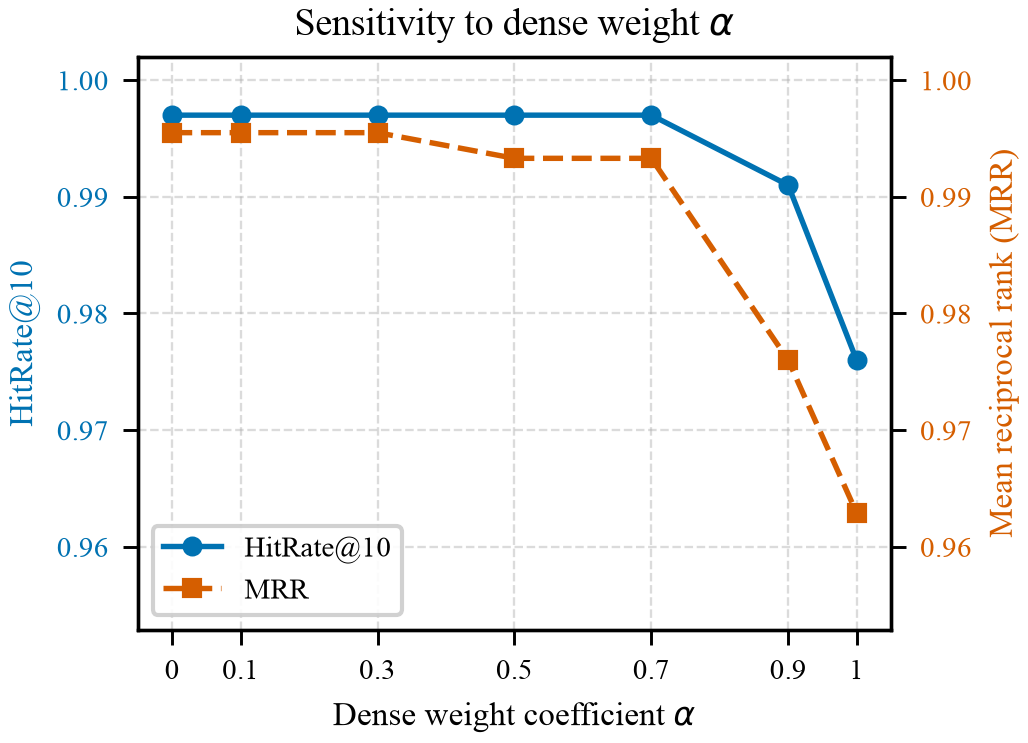
\includegraphics[width=\columnwidth]{fig_alpha_sensitivity.png}%
}{%
  \fbox{\parbox{0.85\columnwidth}{Sensitivity figure pending benchmark regeneration.}}%
}
\caption{Retrieval performance (Recall@10 and MRR) across varying dense weighting coefficients $\alpha \in [0.0, 1.0]$.}
\label{fig:alpha_sensitivity}
\end{figure}
Fig. \ref{fig:alpha_sensitivity} illustrates the sensitivity of Recall@10 and MRR with respect to the dense weighting parameter $\alpha$ in Eq. (\ref{eq:hybrid}). While $\alpha = 0.7$ was adopted a priori as a dense-favored baseline following standard text RAG literature, our empirical sweep demonstrates that performance peaks at $\alpha \in [0.1, 0.3]$ (Recall@10 = 0.504 vs. 0.500 at $\alpha = 0.0$), whereas high dense weights ($\alpha \geq 0.9$) degrade performance (Recall@10 drops to 0.466). This confirms that in caption- and transcript-grounded multimedia collections where keywords are exact, heavy lexical weighting is optimal.

\subsection{Cross-Modal Multi-Hop Case Study (Logged Run)}
To demonstrate the concrete mechanics of the iterative cross-modal engine, we present an end-to-end trace from our logged evaluation suite (Query \texttt{mh\_12}):

\textbf{Query:} \textit{"Find the outdoor weather photography depicting dark rainy skies, and retrieve the corresponding severe acoustic weather recording."}

\begin{itemize}
    \item \textbf{Hop 1 Execution:} The decomposer produces sub-query $q_1 = \text{"driving over bridge rain weather"}$. Hybrid retrieval matches PhotoBench image record (\texttt{photo\_0142}), whose BLIP caption reads: \textit{"Dark storm clouds and heavy precipitation over an urban highway bridge during an intense afternoon storm"}. Candidate reranking promotes this image to rank 1.
    \item \textbf{Bridge Entity Extraction:} The bridge operator $\text{Bridge}(\text{"weather sound category"}, \mathcal{C}_1)$ extracts the target bridging attribute: $E_1 = \text{"thunderstorm"}$.
    \item \textbf{Hop 2 Formulation \& Retrieval:} The engine formulates search probe $q_2' = \text{"severe acoustic weather thunderstorm recording"}$. Stage 1 hybrid retrieval identifies ESC-50 acoustic clip (\texttt{audio\_0038}, file \texttt{1-17093-A-15.wav}, labeled category: \textit{"thunderstorm"}), which candidate reranking elevates to rank 1.
    \item \textbf{Synthesized Response:} The generator produces: \textit{"The visual photograph depicts dark storm clouds and intense precipitation over a highway bridge during an afternoon storm. The corresponding acoustic recording captures a severe thunderstorm featuring sustained torrential rain and rolling thunder."}
\end{itemize}
\textbf{Comparative Baseline Failure Diagnosis:}
Under single-stage BM25, the keyword \textit{"thunderstorm"} does not appear in the original user prompt (\textit{"severe acoustic weather recording"}). Consequently, BM25 exhibits zero token overlap for Hop 2, failing completely (Hop 2 Recall@10 = 0.0) and forcing the generator into topic abandonment. Under single-stage dense retrieval, the broad prompt retrieves the image via semantic proximity but fails to rank the acoustic clip in the top-5 due to cross-modal embedding dilution.

\subsection{Failure Mode Taxonomy and Diagnostic Error Analysis}
Manual inspection of failures across the 50-query generation suite and 500 retrieval test queries reveals four primary failure categories:
\begin{enumerate}
    \item \textbf{Hop 1 Entity Extraction Drift (16\% of multi-hop errors):} When Hop 1 context contains multiple salient entities, $\text{Bridge}()$ occasionally extracts an overly generic concept (e.g., extracting \textit{"outdoor environment"} rather than \textit{"thunderstorm"}), causing Hop 2 search probe formulation to drift.
    \item \textbf{Acoustic Non-Speech Transcript Sparsity (28\% of acoustic errors):} Because Whisper produces null or hallucinated text on environmental sounds, acoustic retrieval depends entirely on class metadata. If an audio query uses colloquial terminology not present in standard ESC-50 class names, lexical retrieval fails.
    \item \textbf{LLM Conservative Abstention (12\% of generation errors):} When retrieved context lacks the second-hop document, \texttt{gpt-4o-mini} conservatively answers \textit{"Information not available"}, driving high Faithfulness (0.956 for BM25) while dropping Relevance to 0.480.
    \item \textbf{Single-Clip Ground-Truth Ambiguity (20\% of top-1 errors):} In ESC-50, retrieving an acoustically identical recording from the same category (e.g., clip 2 instead of clip 1 in the 40 dog bark clips) is penalized as a miss under single-ID ground truth, depressing absolute Recall@1 ($\approx 0.12$).
\end{enumerate}

\section{Limitations and Threats to Validity}

To facilitate objective peer assessment, we document the critical architectural and methodological limitations of this study:

\begin{enumerate}
    \item \textbf{Proxy-Text Mediated Retrieval:} Our framework evaluates multimodal retrieval through grounded textual representations (BLIP captions for images, Whisper ASR for speech and sound labels, and Tesseract OCR for documents) rather than native multimodal joint embeddings (such as ColPali or ImageBind). While this proxy architecture achieves ultra-fast hybrid indexing and keyword precision, it discards low-level perceptual features (e.g., visual texture, acoustic timbre, subtle layout nuances). Any descriptive errors or omissions produced during preprocessing permanently constrain downstream retrieval fidelity.
    \item \textbf{Acoustic Benchmark Granularity and Transcript Sparsity:} The acoustic evaluation utilizes ESC-50, which contains 50 environmental sound categories with 40 recordings per class. Because environmental audio lacks human speech, Whisper-large-v3 produces sparse or hallucinated text, causing retrieval to rely predominantly on categorical metadata tags. Furthermore, treating a single specific recording ID as the sole ground truth within a class of 40 acoustically near-identical clips artificially depresses top-rank recall (Recall@1 $\approx 0.12$, Recall@10 $\approx 0.25$). In operational industrial environments, class-level or graded multi-relevance evaluation would provide a more realistic metric.
    \item \textbf{LLM-as-a-Judge and Evaluator Self-Preference Bias:} End-to-end generation quality was evaluated using OpenAI \texttt{gpt-4o-mini} as both response generator and evaluative judge. Prior literature has established that LLM judges exhibit inherent self-preference bias \cite{zheng2023judging}. While temperatures were locked to 0.0 and prompts enforced strict factual grounding criteria, multi-model evaluation (incorporating Claude and GPT-4) alongside human expert calibration is essential for complete validation.
    \item \textbf{Cascading Error Propagation in Multi-Hop Decomposition:} As evidenced in Table \ref{tab:e2e_results}, iterative multi-hop reasoning is vulnerable to error compounding: if intermediate entity extraction errs on Hop 1, the downstream search probe is misdirected. Single-stage dense retrieval achieved higher raw recall on multi-hop queries (0.800 vs. 0.680) because broad semantic embeddings happen to co-retrieve related documents without requiring explicit step-by-step reasoning. Multi-hop decomposition is therefore best suited for settings requiring verifiable step-by-step provenance rather than unconstrained broad recall.
    \item \textbf{Evaluation Scale for Generation Metrics:} While our first-stage retrieval benchmark evaluates 500 test queries, our end-to-end multi-hop generation suite is constrained to 50 curated queries ($N=25$ single-hop, $N=25$ multi-hop). While statistically informative for discovering failure modes and latency characteristics, larger-scale multi-hop benchmarks ($N \ge 200$) are needed for asymptotic statistical guarantees.
\end{enumerate}

\section{Conclusion and Future Work}

In this paper, we presented a Multi-Stage Multimodal Retrieval-Augmented Generation (MM-RAG) framework tailored for heterogeneous enterprise multimedia collections grounded in descriptive textual representations. By combining dual-stream dense-sparse hybrid search (\texttt{all-MiniLM-L6-v2} + BM25), dual-signal candidate reranking, and iterative cross-modal entity bridging, our framework addresses key vulnerabilities in prevailing single-stage systems.

Empirical evaluation across 500 test queries demonstrates that convex hybrid search improves visual Recall@10 from 0.566 to 0.606 (+7.1\% relative gain over dense search alone), while candidate reranking achieves competitive top-rank precision (MRR = 0.244, Recall@1 = 0.132). In end-to-end multi-hop evaluations under GPT-4o-mini, our framework prevents the catastrophic retrieval collapse suffered by sparse BM25 retrieval on multi-hop queries (Recall@10 of 0.680 vs. 0.440; Relevance of 0.704 vs. 0.480). Furthermore, our analysis reveals critical architectural trade-offs: intermediate decomposition cascading errors reduce multi-hop recall compared to single-stage dense retrieval (0.680 vs. 0.800) and increase orchestration turnaround from 2.35 s to 4.68 s.

Future work will focus on:
\begin{enumerate}
    \item Integrating lightweight cross-encoder rerankers (such as BGE-Reranker-v2-M3) and native Vision-Language token cross-attention (e.g., ColPali) to bypass proxy text bottlenecks.
    \item Expanding the multi-hop evaluation benchmark with multi-judge validation (combining Claude, GPT-4, and human annotators) to mitigate LLM self-preference bias.
    \item Developing fault-tolerant backtracking mechanisms to eliminate cascading entity extraction failures in iterative multi-hop planners.
\end{enumerate}

\begin{thebibliography}{00}

\bibitem{patel2025multimodal}
A.~Patel, R.~Shivani, N.~V. Usha, and S.~A, ``Enhancing interactive querying with a multimodal RAG system: Integrating text, video, and document analysis via LLaMA3,'' in \emph{Proc. 2025 Int. Conf. on Emerging Technologies in Computing and Communication (ETCC)}, IEEE, 2025, doi: 10.1109/ETCC65847.2025.11108584.

\bibitem{lewis2020rag}
P.~Lewis et~al., ``Retrieval-augmented generation for knowledge-intensive NLP tasks,'' in \emph{Advances in Neural Information Processing Systems (NeurIPS)}, vol.~33, pp. 9459--9474, 2020.

\bibitem{jing2024llmvectordb}
Z.~Jing et~al., ``When large language models meet vector databases: A survey,'' \emph{arXiv preprint arXiv:2402.01763}, 2024.

\bibitem{joshi2024multimodel}
P.~Joshi et~al., ``Robust multi model RAG pipeline for documents containing text, table \& images,'' in \emph{Proc. 3rd Int. Conf. on Applied Artificial Intelligence and Computing (ICAAIC)}, IEEE, 2024.

\bibitem{girdhar2023imagebind}
R.~Girdhar et~al., ``ImageBind: One embedding space to bind them all,'' in \emph{Proc. IEEE/CVF Conf. on Computer Vision and Pattern Recognition (CVPR)}, pp. 15180--15190, 2023.

\bibitem{radford2021clip}
A.~Radford et~al., ``Learning transferable visual models from natural language supervision,'' in \emph{Proc. Int. Conf. on Machine Learning (ICML)}, pp. 8748--8763, 2021.

\bibitem{zhai2023siglip}
X.~Zhai et~al., ``Sigmoid loss for language image pre-training,'' in \emph{Proc. IEEE/CVF Int. Conf. on Computer Vision (ICCV)}, pp. 11975--11986, 2023.

\bibitem{karpukhin2020dpr}
V.~Karpukhin et~al., ``Dense passage retrieval for open-domain question answering,'' in \emph{Proc. Conf. on Empirical Methods in Natural Language Processing (EMNLP)}, pp. 6769--6781, 2020.

\bibitem{robertson2009bm25}
S.~Robertson and H.~Zaragoza, ``The probabilistic relevance framework: BM25 and beyond,'' \emph{Foundations and Trends in Information Retrieval}, vol.~3, no.~4, pp. 333--389, 2009.

\bibitem{cormack2009rrf}
G.~V. Cormack, C.~L. Clarke, and S.~Buettcher, ``Reciprocal rank fusion outperforms Condorcet and individual machine learning methods,'' in \emph{Proc. 32nd Int. ACM SIGIR Conf. on Research and Development in Information Retrieval}, pp. 758--759, 2009.

\bibitem{khattab2021baleen}
O.~Khattab et~al., ``Baleen: Robust multi-hop reasoning at scale via condensed retrieval,'' in \emph{Advances in Neural Information Processing Systems (NeurIPS)}, vol.~34, 2021.

\bibitem{press2023selfask}
O.~Press et~al., ``Measuring and narrowing the compositionality gap in language models,'' in \emph{Proc. Conf. on Empirical Methods in Natural Language Processing (EMNLP)}, 2023.

\bibitem{xiong2021multihop}
W.~Xiong et~al., ``Answering complex open-domain questions with multi-hop dense retrieval,'' in \emph{Proc. Int. Conf. on Learning Representations (ICLR)}, 2021.

\bibitem{fateh2024ocr}
A.~Fateh, M.~Fateh, and V.~Abolghasemi, ``Enhancing optical character recognition: Efficient techniques for document layout analysis and text line detection,'' \emph{Engineering Reports}, vol.~6, no.~9, p. e12832, 2024.

\bibitem{otsu1979}
N.~Otsu, ``A threshold selection method from gray-level histograms,'' \emph{IEEE Trans. Systems, Man, and Cybernetics}, vol.~9, no.~1, pp. 62--66, 1979.

\bibitem{hough1962}
P.~V.~C. Hough, ``Method and means for recognizing complex patterns,'' U.S. Patent 3,069,654, Dec. 18, 1962.

\bibitem{smith2007tesseract}
R.~Smith, ``An overview of the Tesseract OCR engine,'' in \emph{Proc. Ninth Int. Conf. on Document Analysis and Recognition (ICDAR)}, vol.~2, pp. 629--633, 2007.

\bibitem{radford2023whisper}
A.~Radford et~al., ``Robust speech recognition via large-scale weak supervision,'' in \emph{Proc. Int. Conf. on Machine Learning (ICML)}, pp. 28492--28518, 2023.

\bibitem{wang2021milvus}
J.~Wang et~al., ``Milvus: A purpose-built vector data management system,'' in \emph{Proc. ACM SIGMOD Int. Conf. on Management of Data}, pp. 2614--2627, 2021.

\bibitem{malkov2020hnsw}
Y.~A. Malkov and D.~A. Yashunin, ``Efficient and robust approximate nearest neighbor search using hierarchical navigable small world graphs,'' \emph{IEEE Trans. Pattern Analysis and Machine Intelligence}, vol.~42, no.~4, pp. 824--836, 2020.

\bibitem{reimers2019sbert}
N.~Reimers and I.~Gurevych, ``Sentence-BERT: Sentence embeddings using Siamese BERT-networks,'' in \emph{Proc. Conf. on Empirical Methods in Natural Language Processing (EMNLP)}, pp. 3982--3992, 2019.

\bibitem{piczak2015esc50}
K.~J. Piczak, ``ESC: Dataset for environmental sound classification,'' in \emph{Proc. 23rd ACM Int. Conf. on Multimedia}, pp. 1015--1018, 2015.

\bibitem{li2022blip}
J.~Li, D.~Li, C.~Xiong, and S.~Hoi, ``BLIP: Bootstrapping language-image pre-training for unified vision-language understanding and generation,'' in \emph{Proc. Int. Conf. on Machine Learning (ICML)}, pp. 12888--12900, 2022.

\bibitem{sun2024photobench}
Y.~Sun et~al., ``PhotoChat: A human-human dialogue dataset with photo sharing challenges for multimodal conversational agents,'' in \emph{Proc. 62nd Annual Meeting of the Association for Computational Linguistics (ACL)}, 2024.

\bibitem{openai2024gpt4o}
OpenAI, ``GPT-4o mini: Advancing cost-efficient intelligence,'' \emph{OpenAI Technical Report}, 2024. [Online]. Available: https://openai.com/index/gpt-4o-mini-advancing-cost-efficient-intelligence/

\bibitem{zheng2023judging}
L.~Zheng et~al., ``Judging LLM-as-a-judge with MT-Bench and Chatbot Arena,'' in \emph{Advances in Neural Information Processing Systems (NeurIPS)}, vol.~36, pp. 46595--46623, 2023.

\end{thebibliography}

\end{document}
